% -------------------------------------------------------------------
\chapter{A placa \textit{CLEAN Arduino Mega}}\label{apendix: clean-arduino-mega-board}
% -------------------------------------------------------------------

A continuação são descritos os principais módulos que compõem a placa CLEAN Arduino Mega e os protótipos desenvolvidos. A Tabela \ref{tab:componentes-clean} mostra os principais componentes de hardware utilizados sem considerar os sensores.

\begin{table}
    \caption{Principais componentes utilizados nos dispositivos CLEAN}
    \label{tab:componentes-clean}
    \centering
    \begin{tabularx}{0.95\textwidth}[h]{
         >{\raggedright\arraybackslash}X
         >{\raggedright\arraybackslash}X 
         >{\raggedright\arraybackslash}X }
        \hline
        \textbf{Item} & \textbf{Descrição} & \textbf{Modelo e fabricante}\\ \hline
        Arduino Mega 2560 & Placa microcontroladora baseada no microcontrolador Microchip ATmega2560 & Arduino MEGA 2560 Rev3, de Arduino\\ \hline
		DS3231 RTC & Relógio em tempo real (RTC) I2C com oscilador de cristal compensado por temperatura integrado & DS3231, by Maxim Integrated\\ \hline
		Soquete micro SD & Soquete TF / micro SD tipo PUSH-PUSH & KLS1-TF-007, da KLS Electronic\\ \hline
        Buffer CI 74XX125 & Portas de buffer de barramento quádruplas com saídas de 3 estados para buffer de pinos de cartão micro SD & 74HC125, da Texas Instruments\\ \hline
        Cartão MicroSD & Cartão Micro SD Classe 10 de 16 GB & microSDHC SanDisk Ultra, da SanDisk\\ \hline
        Módulo GPS & Módulo GPS NEO-6M c/ antena & GY-GPS6MV2, por u-blox\\ \hline
        Módulo GPRS & Shield Arduino - GSM GPRS SIM900 com antena Quad Band & SIM900, da SIMCom\\ \hline
        Módulo Wi-Fi & Módulo serial Wi-Fi ESP-01 ESP8266 & ESP8266, da Expressif\\ \hline
        Sensor BMP280 & Sensor digital de temperatura e pressão BMP280 I2C & BMP280, da Bosch Sensortec\\ \hline
        Sensor SHT20 & Sensor de umidade e temperatura SHT20 I2C & SHT20, por Sensirion\\ \hline
        MAX487 & Transceptor RS-485 MAX487 Baixa potência, taxa de variação limitada & MAX487, da Maxim Integrated\\ \hline
    \end{tabularx}
\end{table}

\section{Módulo de sensoriamento}
\subsection{Sensores}

Nos sistemas desenvolvidos foram utilizados sensores de gases eletroquímicos dos fabricantes \textit{SPEC Sensors} e \textit{Alphasense}.

\subsubsection{Sensores SPEC.}

Os sensores da \textit{SPEC} são sensores amperométricos, constituídos por células eletroquímicas (veja Apêndice \ref{apendix: sensores-ec}) de três eletrodos, i.e.: eletrodos de trabalho, de referência e eletrodo contador. SPEC significa \textit{Screen-Printed Electrochemical}, que é a tecnologia utilizada para a fabricação dos sensores, reduzindo seus custos e dimensões, e ainda mantendo um alto desempenho \cite{SPECSensors2016SPECConsiderations}.

\subsubsection{Sensores Alphasense.}

\textit{Alphasense} fabrica sensores eletroquímicos amperométricos. Especificamente, os sensores da série B4 foram selecionados para os monitores desenvolvidos, já que são indicados pelo fabricante para a medição de baixas concentrações de gases. Estes sensores incorporam um quarto eletrodo, denominado eletrodo auxiliar, que compensa os efeitos da temperatura e da umidade relativa nas leituras dos sensores \cite{Baron2017AmperometricReview}. A Figura \ref{fig:alphasense-b4} ilustra um sensor Alphasense da série B4, suas dimensões e disposição dos eletrodos. Para mais informações sobre os efeitos das variáveis ambientais nas respostas dos sensores, confira a nota de aplicação AAN 110 da Alphasense. Para informações adicionais sobre os sensores da série B4 da Alphasense, como especificações elétricas, dimensões e pinagem, consulte as fichas técnicas dos modelos de sensores listados na Tabela 1.

\begin{figure}
    \centering
    \caption{Sensor de Monôxido de Nitrogênio Alphasense da série B4}
    \begin{center}
        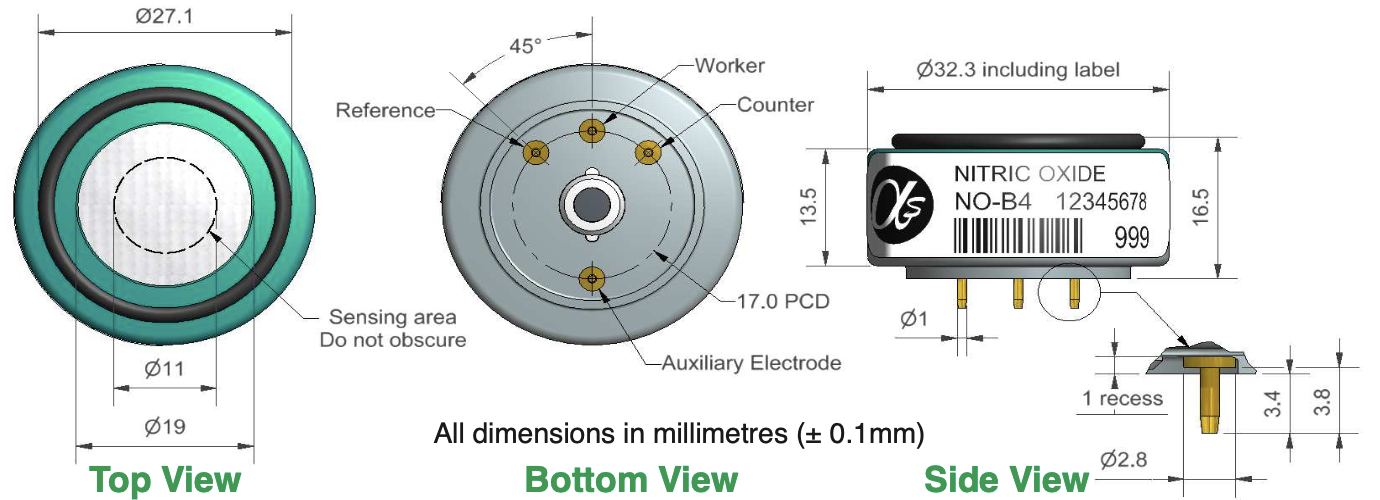
\includegraphics[width=0.75\textwidth]{aftertext/Principais componentes de hardware/Figuras/Sensores serie B4.png}
    \label{fig:alphasense-b4}
	\fonte{\cite{Alphasense2019NO-B4Sensor}.}
    \end{center}
\end{figure}

Sensores eletroquímicos amperométricos produzem uma corrente de saída que é proporcional à concentração do gás. Para ler este sinal elétrico com um sistema de aquisição de dados, a corrente de saída deve ser transformada em um sinal de tensão. Para isso, o circuito mais utilizado é o potenciostato. \textit{Alphasense} e \textit{SPEC} fornecem placas de circuito potenciostato para acoplar facilmente seus sensores a um sistema de monitoramento.

\subsubsection{Interface de condicionamento de sensores SPEC}

Os sensores digitais para IoT fornecidos pela SPEC são compostos por um transdutor eletroquímico montado em uma placa com um circuito potenciostato, que converte a saída do sensor (corrente elétrica) a tensão. Os sensores incorporam também um microcontrolador e um sensor de temperatura e umidade relativa. O microcontrolador adquire o sinal de tensão do potenciostato como valores de concentração de gás e realiza uma compensação em software para reduzir os efeitos da temperatura e a umidade relativa nas leituras do sensor. Os valores de concentração, temperatura e umidade relativa são transmitidos através de uma interface UART seguindo um protocolo serial definido pelo fabricante. Esta placa de condicionamento atua como uma camada de abstração para condicionamento de sinal que permite a fácil integração dos sensores a qualquer sistema de monitoramento. Para obter mais informações sobre os sensores SPEC, como especificações elétricas, dimensões, pinagem e protocolo serial, verifique as fichas técnicas dos sensores (Tabela 1) e do kit de desenvolvimento do sensor de gás digital 968-045 (REF).

\subsubsection{Interface de condicionamento de sensores Alphasense}

A Alphasense fornece placas de sensores individuais para seus sensores de gás de 4 eletrodos da série B4 (REF). Essas placas incorporam circuitos potenciostatos equivalentes para os eletrodos de trabalho e auxiliar. As saídas de cada canal do potenciostato foram conectadas às entradas analógicas do microcontrolador Arduino MEGA, conforme mostrado na Figura A.3. Os sinais AE e WE representam os sinais correspondentes ao eletrodo auxiliar e de trabalho respectivamente. Seis sensores foram utilizados no protótipo, sendo utilizadas assim doze entradas analógicas do microcontrolador (A0 – A11). Cada módulo ISB foi alimentado com uma tensão de 5 V. Para obter mais detalhes sobre a montagem e conexão dos sensores Alphasense, consulte o Guia de montagem de sensores Alphasense.

\section{O microcontrolador}

O microcontrolador Arduino MEGA 2560 coordena as tarefas associadas à aquisição e armazenamento de dados, temporização, geolocalização e comunicação. O firmware para este protótipo está disponível no repositório de firmware. Para obter detalhes sobre a estrutura do firmware e bibliotecas de firmware, consulte a documentação do firmware.

\subsection{Armazenamento dos dados}

Para armazenamento dos dados foi utilizado um módulo micro SD conectado ao microcontrolador através de uma Interface Periférica Serial (SPI). O cartão micro SD funciona com 3.3 V, mas o módulo inclui buffers e um regulador de tensão que permite conexão direta ao Arduino SPI e fonte de alimentação de 5 V, conforme mostra a figura 6.

\subsection{Relógio de tempo real}

Para monitorar a data e a hora de forma contínua foi utilizado o módulo DS1307 Real-Time Clock (RTC). Este módulo é um relógio/calendário de baixo consumo de energia que fornece informações sobre segundos, minutos, horas, dia, data, mês e ano (REF). A data do final do mês é ajustada automaticamente para meses com menos de 31 dias, incluindo correções para anos bissextos. O DS1307 possui um circuito sensor de energia integrado que detecta falhas de energia e alterna automaticamente para a fonte de backup por meio de uma bateria. A operação de cronometragem continua enquanto a peça opera no modo de baixo consumo de energia da fonte de reserva. O módulo se conecta ao Arduino MEGA através da interface I2C e é alimentado com 5V, conforme mostra a figura 7.

\subsection{Comunicação Wi-Fi}

Para a comunicação Wi-Fi foi utilizado o módulo ESP-01 (Figura 8). Este módulo incorpora o microcontrolador ESP8266 junto com uma antena embarcada com ganho de potência de 3dBi e alcance de até 90 m. O ESP8266 é um System on Chip (SoC), fabricado pela Espressif Systems, que integra o microprocessador Tensilica L106 de 32 bits e implementa os protocolos TCP/IP e 802.11 b/g/n WLAN MAC (REF). O ESP-01 também incorpora uma memória flash de 512 kB para programação, que é acessível ao ESP8266 via SPI. Ele também possui oito pinos que são utilizados para alimentação, conexão à porta serial do ESP8266 e conexão aos quatro GPIOs do ESP8266, conforme mostrado na Figura 8. Para mais detalhes sobre a pinagem do ESP-01 e como programar e conectar este módulo para o Arduino MEGA, consulte o Guia de programação do módulo ESP-01. Uma descrição do firmware que desenvolvemos para o microcontrolador ESP8266 pode ser encontrada em The ESP8266 Firmware.

O módulo ESP-01 fornece a conexão a uma rede Wi-Fi para o Arduino MEGA. Conforme mostrado na Figura 9, um circuito de mudança de nível é necessário para fazer a interface com os pinos do Arduino como resultado das diferentes tensões de operação das placas. A comunicação entre os microcontroladores ATMega2560 e ESP8266 é implementada através de uma interface UART (UART3 na placa Arduino), seguindo um protocolo de comunicação que é descrito detalhadamente no Guia de Programação do Módulo ESP-01. O Arduino atua como mestre do ESP8266, cuja única iniciativa é estabelecer conexão com a Internet. Uma vez estabelecida a conexão, o Arduino pode enviar comandos para criar posts HTTP, obter o horário da internet ou obter as coordenadas de geolocalização do Google; para obter mais detalhes, consulte o Guia de programação do módulo ESP-01. O microcontrolador Arduino também pode redefinir o ESP8266 através do pino D12 GPIO.